\lab{Transit time crossing a river}{Transit time crossing a river}
\label{lab:rivercrossing}
\objective{This lab discusses a classical calculus of variations problem: how is a river to be crossed in the shortest possible time? 
We will look at a numerical solution using the pseudospectral method. }

Suppose a boat is to be rowed across a river, from a point $A$ on one side of a river ($x=-1$), to a point $B$ on the other side ($x=1$). 
Assuming the boat moves at a constant speed 1 relative to the current, how must the boat be steered to minimize the time required to cross the river? 

\begin{figure}
\centering
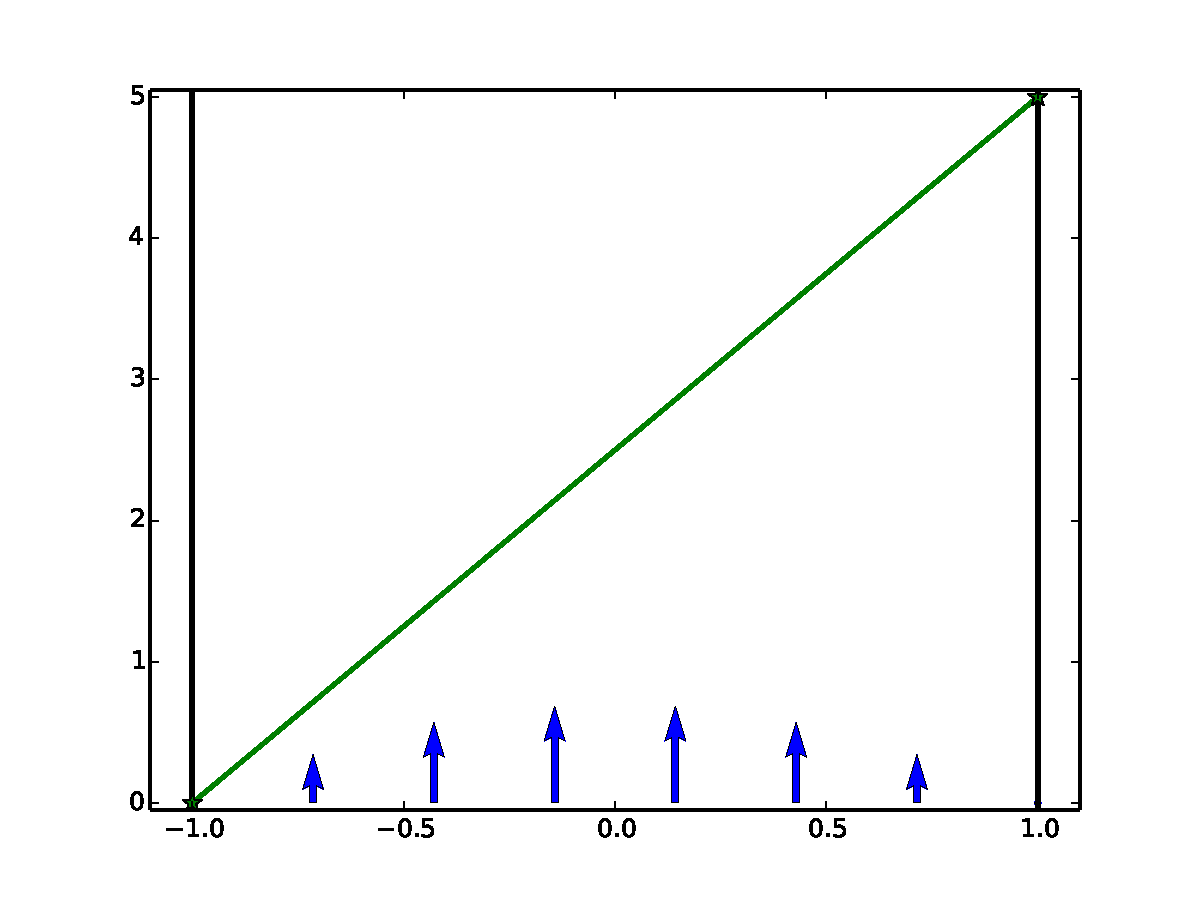
\includegraphics[width=\textwidth]{rivercurrent.pdf}
\caption{The river's current, along with a possible trajectory for the boat.}
\label{fig:rivercrossing_current}
\end{figure}

Let us consider a typical trajectory for the boat as it crosses the river. 
If $T$ is the time required to cross the river, then the position $s$ of the boat at time $t$ is
\begin{align*}
	s(t) &= \langle x(t), y(t) \rangle, \quad t \in [0,T], \\
	s'(t) &= \langle x'(t), y'(t) \rangle, \\
	&= \langle \cos \theta(x(t)),\sin \theta(x(t)) \rangle + \langle 0, c(x(t)) \rangle.
\end{align*}
Here $\langle \cos \theta, \sin \theta \rangle$ represents the motion of the boat due to the rower, and $\langle 0, c \rangle$ is the motion of the boat due to the current.

We can relate the angle at which the boat is steered to the graph of its trajectory by noting that 
\begin{align}
\begin{split}
	y'(x) &= \frac{y'(t)}{x'(t)} ,\\
	&= \frac{\sin \theta + c}{\cos \theta},\\
	&= c\sec \theta + \tan \theta .%, \\
	% &= c \sec \theta + \sqrt{\sec^2 \theta -1}.
\end{split} \label{rivercrossing:angle}
\end{align}
The time $T$ required to cross the river is given by
\begin{align}
\begin{split}
	T &= \int_{-1}^1 t'(x)\, dx, \\
	&= \int_{-1}^1 \frac{1}{x'(t)}\, dx \\ 
	&= \int_{-1}^1 \sec \theta (x)\, dx. 
\end{split}\label{rivercrossing:T}
\end{align}
We would like to find an expression for the total time $T$ required to cross the river from $A$ to $B$, in terms of the graph of the boat's trajectory. 
To derive the functional $T[y]$, we note that 
\begin{align*}
	T[y] &= \int_{-1}^1 \sec \theta\, dx,\\
	&= \int_{-1}^1 \frac{1}{1-c^2}(c \tan \theta + \sec \theta -c^2 \sec \theta - c\tan \theta)\, dx, \\
	&= \int_{-1}^1 \frac{1}{1-c^2}(c \tan \theta + \sec \theta -c y' )\, dx.	
\end{align*}
Since 
\begin{align*}
	c\tan \theta + \sec \theta &= \sqrt{1 - c^2 + (c \sec \theta + \tan \theta)^2},\\
	&= \sqrt{1 - c^2 + (y')^2},
\end{align*}
we obtain at last
\begin{align}
	T[y] &= \int_{-1}^1 \left[ \alpha(x)\sqrt{1 + (\alpha y')^2(x)} - (\alpha^2 c y')(x) \right]\, dx,
\end{align}
where $\alpha = (1 - c^2)^{-1/2}$.

\begin{problem}
Assume that the current is given by $c(x) = -.7(x-1)(x+1)$. (This function assumes, for example, that the current is faster near the center of the river.)
Write a Python function that accepts as arguments a function $y$, its derivative $y'$, and an $x$-value, and returns $L(x,y(x),y'(x))$ (where $T[y] = \int_{-1}^1 L(x,y(x),y'(x))$). Use that function to define a second function that numerically computes $T[y]$ for a given path $y(x)$. 
\end{problem}

\begin{problem}
	Let $y(x)$ be the straight-line path between $A = (-1,0)$ and $B=(1,5)$. Numerically calculate $T[y]$ to get an upper bound on the minimum time required to cross from $A$ to $B$. Using $\eqref{rivercrossing:T}$, find a lower bound on the minimum time required to cross.
\end{problem}

We look for the path $y(x)$ that minimizes the time required for the boat to cross the river, so that the function $T$ is minimized. From the calculus of variations we know that a smooth path $y(x)$ minimizes $T$ only if the Euler-Lagrange equation is satisfied. Recall that the Euler-Lagrange equation is 
\[
% \frac{\partial }{\partial y}L - \frac{d}{dx}\frac{\partial }{\partial y'}L
L_{y} - \frac{d}{dx}L_{y'} = 0.
\]
Since $L_y = 0$, we see that the shortest time trajectory satisfies
\begin{align*}
	\frac{d}{dx}L_{y'} &=  \frac{d}{dx}\left( \alpha^3(x) y'(x) (1 + (\alpha y')^2(x))^{-1/2} - \alpha^2(x) c \right) = 0.
\end{align*}

\begin{problem}
Using the pseudospectral method, calculate the numerical solution of the Euler-Lagrange equation satisfying the boundary conditions $y(-1) = 0$, $y(1) = 5$. (Hint: Replace each $\frac{d}{dx}$ with the differentiation matrix $D$. Then impose the boundary conditions and solve.)
\end{problem}

\begin{problem}
Plot the angle at which the boat should be pointed at each $x$-coordinate. (Hint: Use  Equation \eqref{rivercrossing:angle}; see Figure \ref{fig:rivercrossing_angle}. Note that the angle the boat should be steered is \emph{not} described by the tangent vector to the trajectory.)

\end{problem}

\begin{figure}
\centering
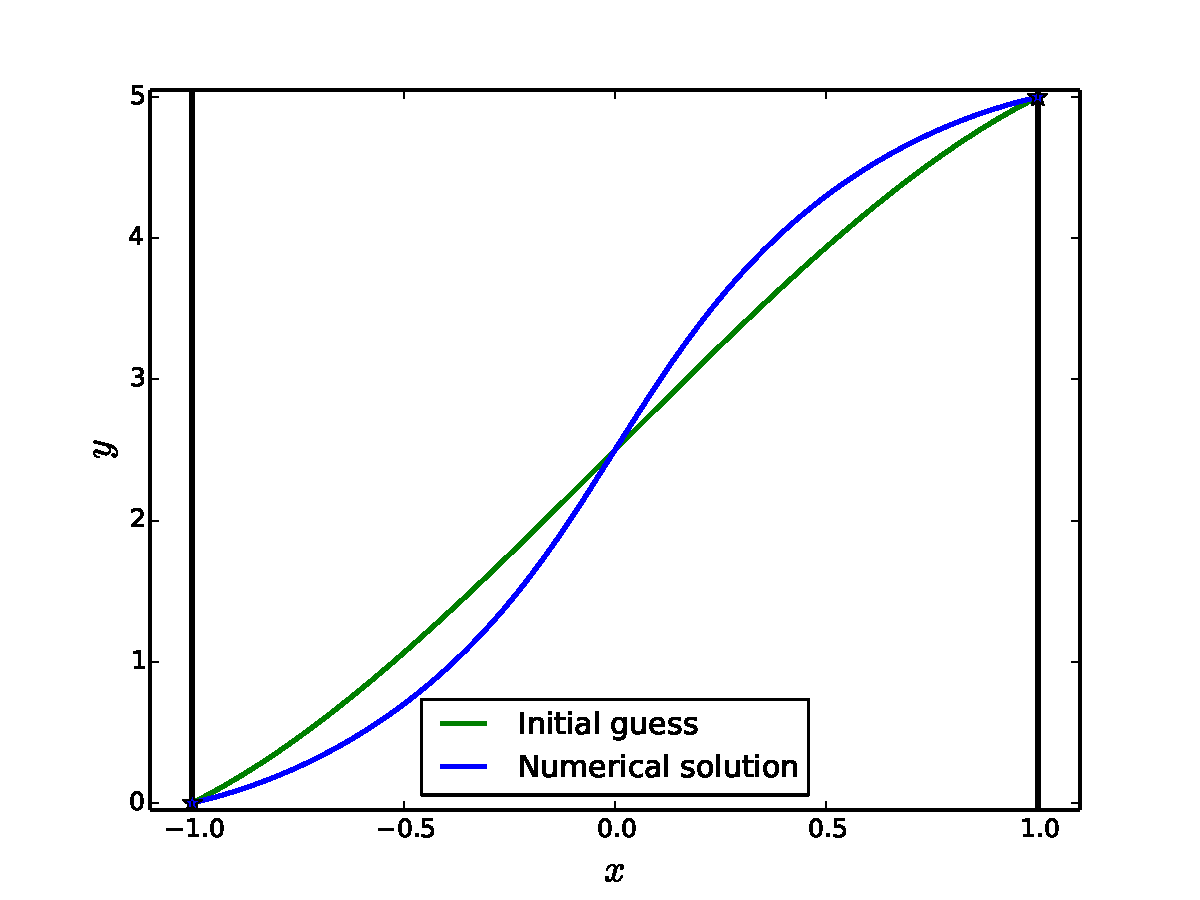
\includegraphics[width=\textwidth]{minimum_time_rivercrossing.pdf}
\caption{Numerical computation of the trajectory with the shortest transit time.}
\label{fig:rivercrossing_trajectory}
\end{figure}



\begin{figure}
\centering
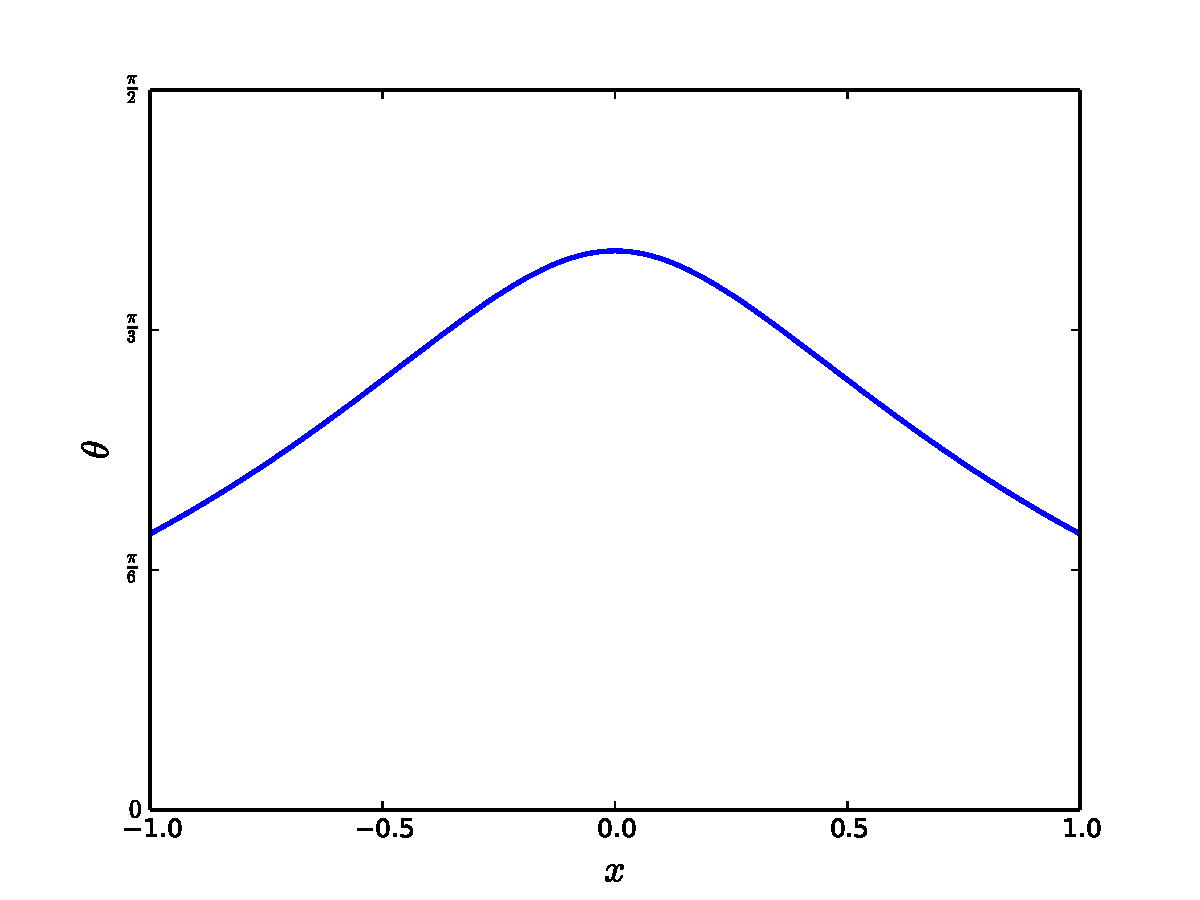
\includegraphics[width=\textwidth]{trajectory_angle.pdf}
\caption{The optimal angle to steer the boat.}
\label{fig:rivercrossing_angle}
\end{figure}






